\documentclass[a4paper, 12pt]{article}
\usepackage[utf8]{inputenc}
\usepackage{amsmath}
\usepackage{amsfonts}
\usepackage{graphicx}
\usepackage{hyperref}
\usepackage{float}
%\usepackage{tikz}
%\usetikzlibrary{positioning}

\title{Apprentissage par Renforcement pour le Contrôle d'un Drone}
\author{Inès Hafassa-Maïza, Hugo Laval}
\date{\today}

\begin{document}

\maketitle



\begin{figure}[H]
    \centering
    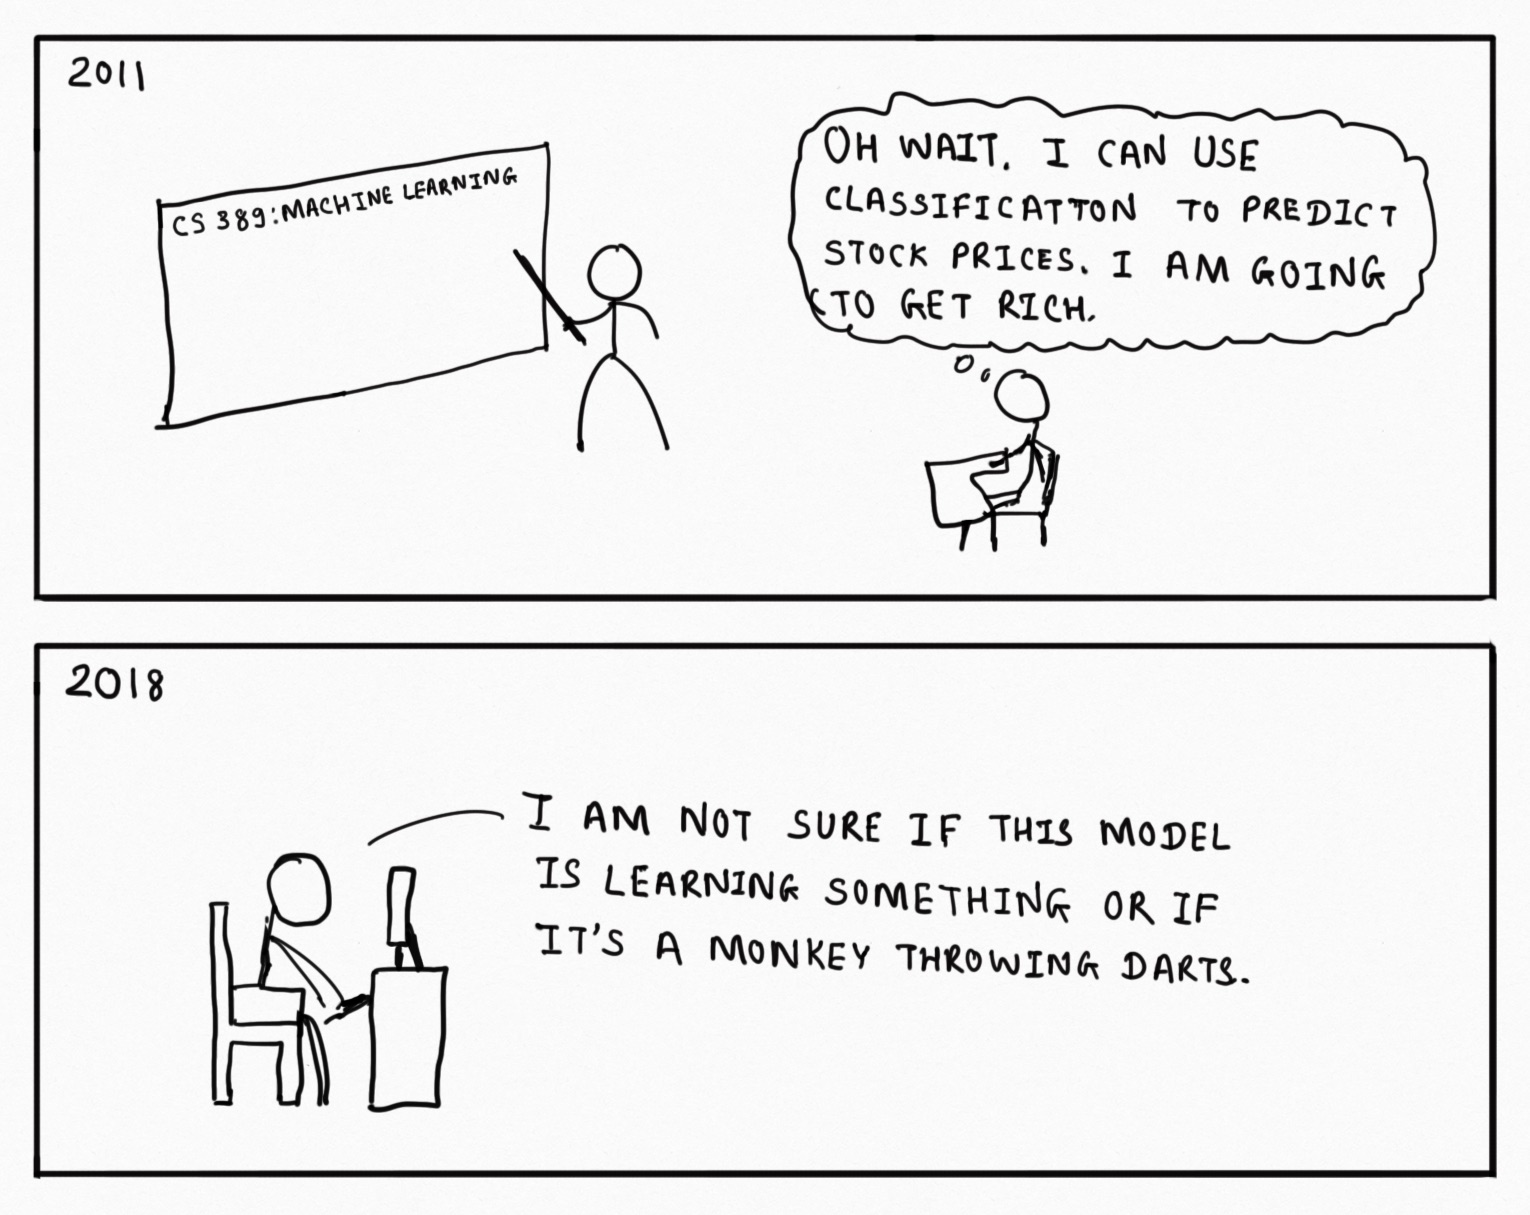
\includegraphics[width=0.8\textwidth]{ml_class_sketch.jpg}
    \caption{Hardik Patel}
\end{figure}
\newpage
\tableofcontents
\newpage


\section{Introduction}
Ce rapport décrit l'utilisation de l'apprentissage par renforcement pour contrôler un drone dans un environnement 3D avec des obstacles. Le but est de permettre au drone de naviguer de manière autonome vers une destination tout en évitant les obstacles.

\section{Mise en place de l’environnement}

Nous avons défini un environnement tridimensionnel dans lequel évolue notre drone. Cet environnement est représenté par un cube de côté 10 contenant des obstacles sphériques de tailles variables, générés aléatoirement.

Afin de simuler des conditions réalistes, la position initiale du drone et sa destination sont sélectionnées de manière aléatoire selon une distribution uniforme. Nous nous assurons que ces points ne se situent pas à l’intérieur d’un obstacle afin de garantir des trajectoires réalisables.

Le drone est modélisé par une sphère de volume $\epsilon$. On considère qu’il a atteint sa destination avec succès si la distance euclidienne entre son centre et le point d’arrivée est inférieure à $\epsilon$. Inversement, si cette distance devient inférieure à $\epsilon$ par rapport à un obstacle, la mission est considérée comme un échec.

Pour naviguer en toute sécurité, le drone est équipé de radars omnidirectionnels lui permettant de détecter les obstacles dans un rayon de 10 unités selon la norme L2 dans $\mathbb{R}^3$. Il avance par pas de distance fixe et ajuste sa trajectoire en fonction des obstacles détectés. Par défaut, il se dirige en ligne droite vers sa cible mais, en présence d’un obstacle dans son champ de détection, il adapte sa trajectoire grâce à un algorithme d’apprentissage par renforcement de type Actor-Critic, détaillé ultérieurement.

L’environnement est structuré selon des règles spécifiques pour la génération des obstacles. Le nombre d’obstacles est tiré aléatoirement selon une loi uniforme discrète entre 0 et 10. Les centres des obstacles sont générés aléatoirement dans le cube, chaque coordonnée $(x, y, z)$ suivant une loi uniforme $U(0, 10)$. Les rayons des obstacles sont déterminés aléatoirement selon une loi uniforme continue entre 0.5 et 2.5.

Ce processus garantit une distribution aléatoire des obstacles et permet de générer des scénarios diversifiés pour entraîner le drone à naviguer efficacement dans des environnements dynamiques et imprévisibles.

\section{Formulation du Problème}
Le problème est formulé comme un processus de décision markovien (MDP) défini par l'ensemble $(S, A, P, R, \gamma)$ où :
\begin{itemize}
    \item $S$ est l'ensemble des états, représentant la position, la vitesse, la batterie du drone et la destination finale. Plus précisément, $S \subseteq \mathbb{R}^{10}$, où chaque état est un vecteur de dimension 10 comprenant les coordonnées $(x, y, z)$ de la position, les composantes $(Vx, Vy, Vz)$ de la vitesse, le niveau de batterie $B$, et les coordonnées $(x_d, y_d, z_d)$ de la destination.
    \item $A$ est l'ensemble des actions, représentant les accélérations possibles du drone dans les trois directions de l'espace. Plus précisément, $A \subseteq \mathbb{R}^3$, où chaque action est un vecteur de dimension 3 comprenant les composantes $(Ax, Ay, Az)$ de l'accélération.
    \item $P$ est la fonction de transition d'état, définissant la probabilité de passer d'un état à un autre après une action. $P : S \times A \times S \rightarrow [0, 1]$ est une distribution de probabilité sur les états futurs donnée l'état actuel et l'action choisie.
    \item $R$ est la fonction de récompense, définissant la récompense reçue après chaque transition. $R : S \times A \rightarrow \mathbb{R}$ est une fonction qui attribue une valeur réelle à chaque paire état-action, représentant la récompense immédiate obtenue.
    \item $\gamma$ est le facteur de discount, représentant l'importance des récompenses futures. $\gamma \in [0, 1]$ est un scalaire qui pondère les récompenses futures par rapport aux récompenses immédiates.
\end{itemize}

L'objectif est de trouver une politique $\pi(a|s)$ qui maximise la récompense cumulée attendue :
\[
G_t = \mathbb{E} \left[ \sum_{k=0}^{\infty} \gamma^k R_{t+k+1} \mid S_t = s \right]
\]

\section{Fonction de Récompense}
La fonction de récompense est un élément crucial dans l'apprentissage par renforcement, car elle guide l'agent (le drone) vers un comportement optimal. Dans notre implémentation, la fonction de récompense est conçue pour encourager le drone à atteindre sa destination tout en évitant les obstacles. Si le drone atteint sa destination, une récompense élevée de 1000 est attribuée. En revanche, une pénalité sévère de -500 est appliquée en cas de collision avec un obstacle. De plus, pour chaque mouvement, une récompense proportionnelle à la réduction de la distance par rapport à la destination est calculée, incitant le drone à se rapprocher de son objectif. Une pénalité énergétique est également appliquée pour chaque action, proportionnelle à la racine de l'accélération utilisée, afin de simuler la consommation de la batterie.

Les variables d'état du drone sont modélisées comme suit :
\begin{itemize}
    \item $X_t=(x_t, y_t, z_t) \in [0, 10]$ représentent les coordonnées de la position du drone à l'instant $t$.
    \item $(Vx_t, Vy_t, Vz_t) \in \mathbb{R}$ représentent les composantes de la vitesse du drone à l'instant $t$.
    \item $B_t \in [0, 10000]$ représente le niveau de batterie du drone à l'instant $t$.
\end{itemize}

Nous définissons également :
\begin{itemize}
    \item $\mathcal{O}$ : l'ensemble des obstacles.
    \item $X_{d}=(x_d,y_d,z_d) \in [0,10] \setminus O$ : le point de livraison.
   
\end{itemize}

La fonction de coût $C_t$ à minimiser est définie comme suit :
\[
C_t = -R_t = 
-1000 \cdot \mathbf{1}_{\{X_t = X_d\}} + 500 \cdot \mathbf{1}_{\{X_t \in \mathcal{O}\}} + 1000 \cdot \mathbf{1}_{\{B_t = 0\}} - \alpha \left\| X_{t+1} - X_t \right\|_2 + \beta \left\| A_t \right\|_2
\]
où $\alpha$ et $\beta$ sont des coefficients de pondération pour la distance parcourue et la consommation d'énergie, respectivement, et $A_t = (Ax_t, Ay_t, Az_t)$ représente les composantes de l'accélération appliquée au drone à l'instant $t$.
\newpage
\section{Modèle Actor-Critic}
Lorsque le drone est incapable d'aller vers sa destination en ligne droite car un obstacle se trouve sur sa route, le modèle Actor-Critic est alors utilisé. Il combine deux réseaux de neurones :
\begin{itemize}
    \item L'actor, qui propose des actions basées sur les états actuels.
    \item Le critic, qui évalue la qualité des actions proposées en estimant la valeur des états.
\end{itemize}

\subsection{Fonctionnement}
Le réseau Actor-Critic fonctionne en deux étapes :
\begin{enumerate}
    \item L'actor prend un état $s$ et propose une action $a$ en suivant une politique $\pi(a|s)$.
    \item Le critic évalue cette action en calculant la valeur de l'état $V(s)$ et l'avantage $A(s, a)$.
\end{enumerate}
\begin{figure}[h]
    \centering
    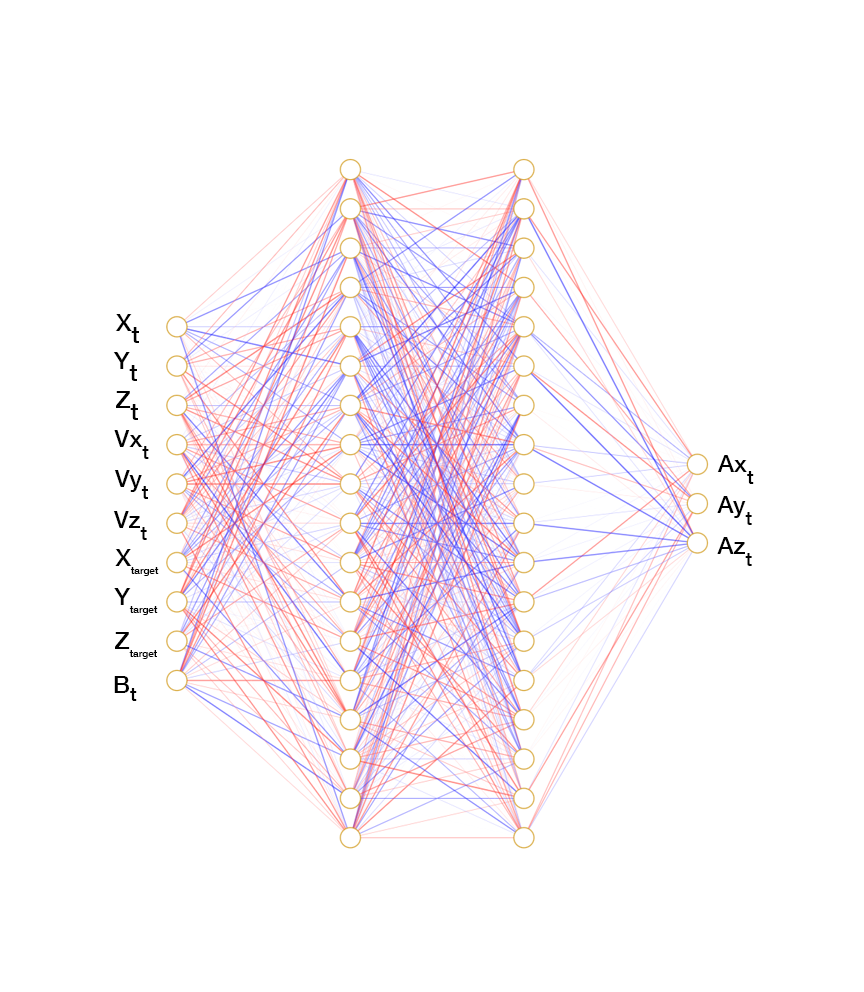
\includegraphics[width=0.5\textwidth]{actor_cnn.png}
    \caption{Architecture du réseau de neuronnes pour l'Actor}
    \label{fig:actor-critic}
\end{figure}

\subsection{Fonction Objectif}
L'objectif de l'algorithme Actor-Critic est une combinaison du gradient de politique (pour l'actor) et de la fonction de valeur (pour le critic). La fonction objectif globale est généralement exprimée comme la somme de deux composants :
\begin{itemize}
    \item \textbf{Gradient de Politique (Actor)} :
    \[
    \nabla_\theta J(\theta) \approx \frac{1}{N} \sum_{i=0}^{N} \nabla_\theta \log \pi_\theta(a_i \mid s_i) \cdot A(s_i, a_i)
    \]
    où $J(\theta)$ représente le retour attendu sous la politique paramétrée par $\theta$, $\pi_\theta(a \mid s)$ est la fonction de politique, $N$ est le nombre d'expériences échantillonnées, $A(s, a)$ est la fonction d'avantage représentant l'avantage de prendre l'action $a$ dans l'état $s$, et $i$ représente l'index de l'échantillon.
    \item \textbf{Mise à Jour de la Fonction de Valeur (Critic)} :
    \[
    \nabla_w J(w) \approx \frac{1}{N} \sum_{i=1}^{N} \nabla_w (V_w(s_i) - Q_w(s_i, a_i))^2
    \]
    où $\nabla_w J(w)$ est le gradient de la fonction de perte par rapport aux paramètres du critic $w$, $V_w(s_i)$ est l'estimation du critic de la valeur de l'état $s$ avec le paramètre $w$, et $Q_w(s_i, a_i)$ est l'estimation du critic de la valeur de l'action $a$.
\end{itemize}

\subsection{Fonction d'Avantage}
La fonction d'avantage, $A(s, a)$, mesure l'avantage de prendre l'action $a$ dans l'état $s$ par rapport à la valeur attendue de l'état sous la politique actuelle :
\[
A(s, a) = Q(s, a) - V(s)
\]
où $Q(s, a)$ est la valeur de l'action et $V(s)$ est la valeur de l'état.

\subsection{Avantages de l'Algorithme Actor-Critic}
L'algorithme Actor-Critic offre plusieurs avantages :
\begin{itemize}
    \item \textbf{Efficacité de l'Échantillon Améliorée} : La nature hybride des algorithmes Actor-Critic conduit souvent à une meilleure efficacité de l'échantillon, nécessitant moins d'interactions avec l'environnement pour atteindre des performances optimales.
    \item \textbf{Convergence Plus Rapide} : La capacité de la méthode à mettre à jour simultanément la politique et la fonction de valeur contribue à une convergence plus rapide pendant l'entraînement, permettant une adaptation plus rapide à la tâche d'apprentissage.
    \item \textbf{Polyvalence à Travers les Espaces d'Action} : Les architectures Actor-Critic peuvent gérer de manière transparente les espaces d'action discrets et continus, offrant une flexibilité pour aborder une large gamme de problèmes d'apprentissage par renforcement.
    \item \textbf{Apprentissage Hors-Politique (dans certaines variantes)} : Apprend à partir d'expériences passées, même lorsqu'elles ne suivent pas directement la politique actuelle.
\end{itemize}

\section{Implémentation}

Pour implémenter la simulation du déplacement du drone dans un environnement 3D, nous avons défini plusieurs classes et fonctions dans le fichier \texttt{knows\_destination2.py}. Parmi celles-ci, les méthodes \texttt{move} et \texttt{step} jouent un rôle essentiel dans la gestion du mouvement du drone et son interaction avec l’environnement.

\subsection{Déplacement du Drone}

Le déplacement du drone est assuré par deux méthodes principales :
\begin{itemize}
    \item \texttt{move} : mise à jour de la position du drone en fonction de l’action choisie.
    \item \texttt{step} : gestion de l’interaction du drone avec son environnement.
\end{itemize}

\subsubsection{Méthode \texttt{move}}

La méthode \texttt{move} prend en entrée :
\begin{itemize}
    \item \texttt{action} : un vecteur représentant l’accélération appliquée au drone.
\end{itemize}

Elle exécute les opérations suivantes :
\begin{enumerate}
    \item \textbf{Vérification de l’arrivée} : si le drone est à une distance inférieure ou égale à $\epsilon$ de la destination, il cesse tout déplacement puisqu'il est arrivé.
    %\item \textbf{Limitation et normalisation de l’action} : l’action est contrainte à l’intervalle $[-1,1]$ pour éviter des valeurs extrêmes et est ensuite normalisée à une norme de 1.
    \item \textbf{Mise à jour de l’accélération et de la vitesse} : l’accélération du drone est mise à jour en fonction de l’action reçue, puis la vitesse est ajustée.
    \item \textbf{Calcul de la nouvelle position} : la nouvelle position est obtenue en ajoutant la vitesse actuelle à la position précédente.
    \item \textbf{Vérification des limites} : si la nouvelle position se trouve à l’intérieur des frontières du cube de simulation dans aucun obstacle, elle est validée.
    \item \textbf{Consommation d’énergie} : la batterie du drone est réduite en fonction de l’accélération appliquée.
\end{enumerate}

\subsubsection{Méthode \texttt{step}}

La méthode \texttt{step} prend en entrée :
\begin{itemize}
    \item \texttt{action} : un vecteur d’accélération choisi par le drone ou calculé par l’algorithme Actor-Critic.
\end{itemize}

Elle suit les étapes suivantes :
\begin{enumerate}
    \item \textbf{Calcul de la direction idéale} : le vecteur directionnel optimal vers la destination est déterminé.
    \item \textbf{Gestion des obstacles} : si aucun obstacle n’est détecté dans cette direction, le drone suit ce chemin ; sinon, l’algorithme Actor-Critic génère une nouvelle action pour éviter l’obstacle.
    \item \textbf{Mise à jour de la position} : la méthode \texttt{move} est appelée pour appliquer l’action et modifier la position du drone.
    \item \textbf{Vérification des conditions d’arrêt} : l’épisode se termine si :
    \begin{itemize}
        \item le drone atteint la destination,
        \item le drone heurte un obstacle,
        \item la batterie est épuisée.
    \end{itemize}
    \item \textbf{Calcul de la récompense} : la récompense est attribuée en fonction de plusieurs critères :
    \begin{itemize}
        \item la distance parcourue vers la cible,
        \item l’évitement des obstacles,
        \item l’efficacité énergétique.
    \end{itemize}
    \item \textbf{Retour des informations} : la méthode retourne l’état actuel du drone, la récompense obtenue, un indicateur de fin d’épisode et des informations complémentaires.
\end{enumerate}

Ces méthodes permettent au drone de naviguer de manière autonome dans l’environnement 3D en optimisant sa trajectoire et en évitant les obstacles grâce à l’apprentissage par renforcement.

\subsection{Entraînement}
Dans un premier temps, nous avons entraîné le drone en le plaçant dans un environnement généré aléatoirement, où il doit atteindre une cible également générée de manière aléatoire. Ce processus est répété un grand nombre de fois, correspondant au nombre d'époques d'entraînement. À chaque fois que le drone réussit ou échoue, l'environnement est réinitialisé de manière aléatoire.

Cette approche a conduit à des comportements très efficaces lorsque la cible est visible en ligne droite, comme illustré à la figure 2. Cependant, l'algorithme s'avère moins performant lorsqu'il s'agit d'esquiver des obstacles. Le drone parvient à s'éloigner de l'obstacle, mais il semble incapable de retrouver la direction de la cible une fois qu'il a modifié sa trajectoire pour éviter l'obstacle (voir figure 3).
\begin{table}[H]
    \centering
    \begin{tabular}{|c|c|}
        \hline
        \textbf{Paramètre} & \textbf{Valeur} \\
        \hline
        Nombre d'époques & 10 \\
        Rayon de détection & 2 \\
        $\epsilon$ & 0.5 \\
        Taille des pas & 0.2 \\
        \hline
    \end{tabular}
    \caption{Paramètres d'entraînement du drone}
    \label{tab:training-parameters}
\end{table}
\begin{figure}[H]
    \centering
    \begin{minipage}{0.49\textwidth}
        \centering
        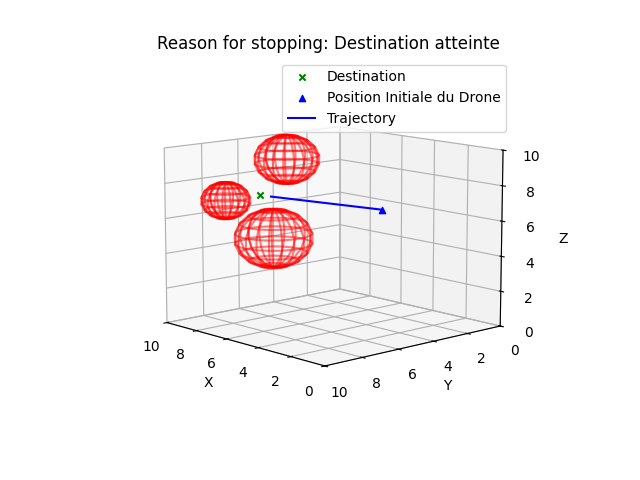
\includegraphics[width=\textwidth]{Figure_7.png}
    \end{minipage}
    \hfill
    \begin{minipage}{0.49\textwidth}
        \centering
        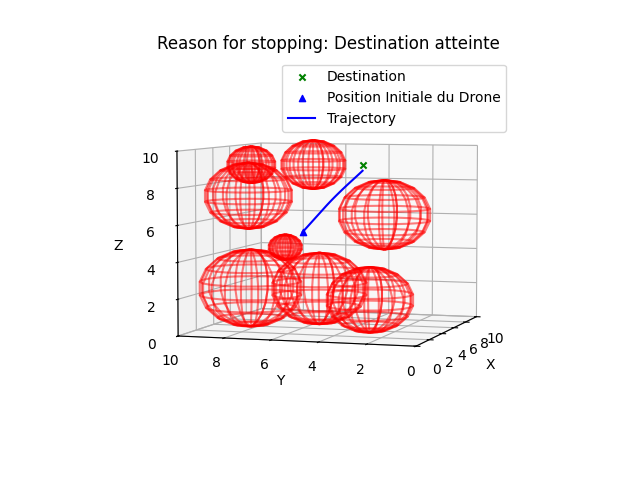
\includegraphics[width=\textwidth]{Figure_8.png}
    \end{minipage}
    \caption{Trajectoire du drone vers la cible avec obstacles sur la trajectoire}
\end{figure}

\begin{figure}[H]
    \centering
    \begin{minipage}{0.49\textwidth}
        \centering
        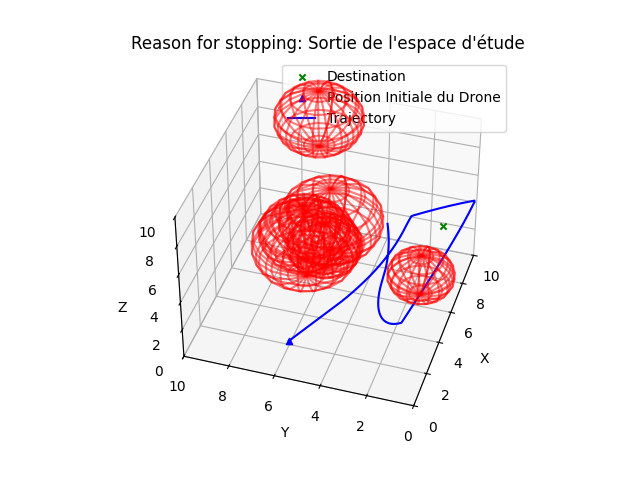
\includegraphics[width=\textwidth]{Figure_9.png}
    \end{minipage}
    \hfill
    \begin{minipage}{0.49\textwidth}
        \centering
        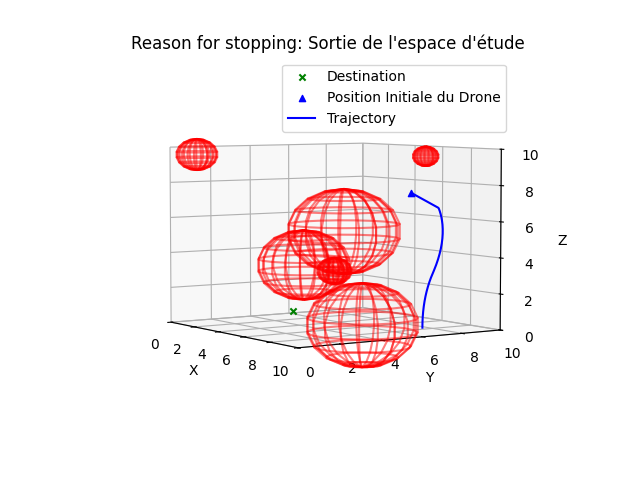
\includegraphics[width=\textwidth]{Figure_10.png}
    \end{minipage}
    \caption{Trajectoire du drone vers la cible avec obstacles sur la trajectoire}
\end{figure}
\section{Modification de l'objectif}

Pour améliorer les performances du drone dans l'évitement d'obstacles, nous avons décidé de l'entraîner spécifiquement à cette tâche. Désormais, le drone évolue dans le même environnement avec la même position de départ et la même cible pour chaque épisode de l'entraînement. Nous nous assurons qu'il y ait toujours un obstacle sur la route directe en direction de la cible pour obliger le drone à l'éviter. Cela améliore la capacité d'évitement comme on peut le constater sur la figure 4.
\begin{table}[H]
    \centering
    \begin{tabular}{|c|c|}
        \hline
        \textbf{Paramètre} & \textbf{Valeur} \\
        \hline
        Nombre d'époques & 10 \\
        Rayon de détection & 2 \\
        $\epsilon$ & 0.5 \\
        Taille des pas & 0.2 \\
        \hline
    \end{tabular}
    \caption{Paramètres d'entraînement spécifiques à l'évitement d'obstacles}
    \label{tab:training-parameters}
\end{table}
\begin{figure}[H]
    \centering
    \begin{minipage}{0.49\textwidth}
        \centering
        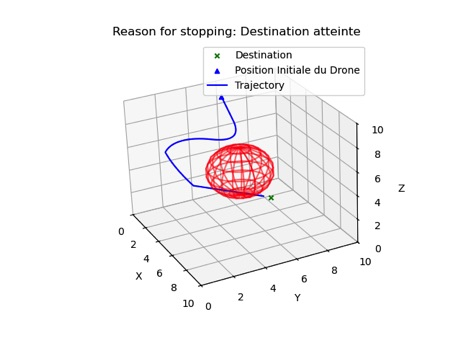
\includegraphics[width=\textwidth]{att.D1KL_7bUX90t0ksXRxzEPxHcgLQs8o7jh7mdn5SYMgo.png}
    \end{minipage}
    \hfill
    \begin{minipage}{0.49\textwidth}
        \centering
        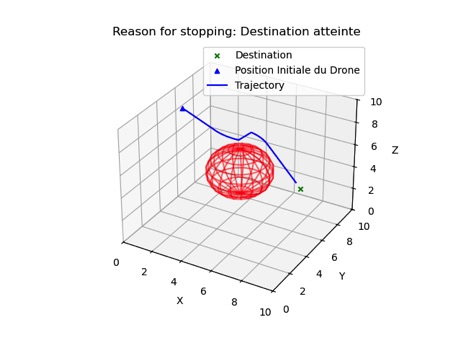
\includegraphics[width=\textwidth]{traj_evite.png}
    \end{minipage}
    \caption{Trajectoire avec obstacles sur la trajectoire et entraînement spécifique}
\end{figure}

\begin{figure}[H]
    \centering
    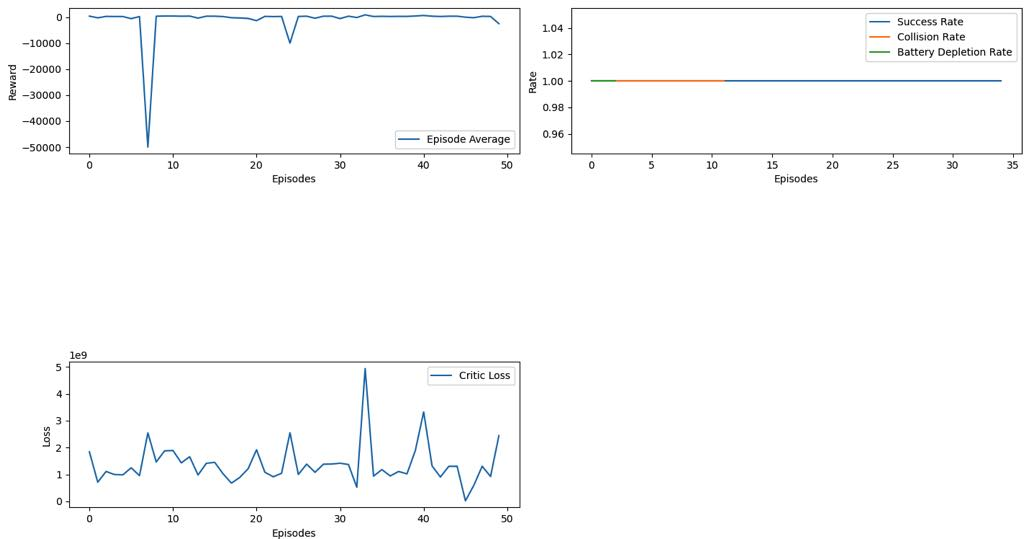
\includegraphics[width=0.8\textwidth]{metrics.png}
    \caption{Quelques métriques d'évaluation}
\end{figure}

\section{Conclusion}

En conclusion, l'apprentissage par renforcement avec le modèle Actor-Critic s'est révélé être une approche efficace pour le contrôle autonome de drones dans des environnements complexes. En entraînant le drone à naviguer vers une cible tout en évitant les obstacles, nous avons pu observer une amélioration significative de ses capacités de navigation et d'évitement. Les résultats montrent que le drone peut apprendre à optimiser sa trajectoire et à gérer efficacement les obstacles grâce à l'entraînement spécifique. Cette méthode offre une solution prometteuse pour des applications futures dans des environnements réels où la navigation autonome est essentielle.

En guise d'amélioration, nous aurions pu essayer d'entraîner le modèle sur des obstacles non convexes, ce qui complexifie la minimisation de la fonction objectif. Nous pourrions aussi essayer d'éviter des obstacles qui sont eux-mêmes en mouvement, comme pour simuler des oiseaux ou d'autres agents dans le ciel. Nous avons pris beaucoup de plaisir à réaliser ce projet et regrettons de ne pas avoir eu plus de temps pour l'améliorer.

\section{Références}

\begin{thebibliography}{9}

\bibitem{geeksforgeeks}
GeeksforGeeks, \textit{Actor-Critic Algorithm in Reinforcement Learning}, [Online]. Available: \url{https://www.geeksforgeeks.org/actor-critic-algorithm-in-reinforcement-learning/}. [Accessed: 10-Feb-2025].

\bibitem{PrivatMoyal2024}
Y. Privat and P. Moyal, \textit{Cours d'apprentissage par renforcement}, M2 IMSD, Mines Nancy/Université de Lorraine, 2024.

\bibitem{wikipedia2024}
\textit{Algorithme acteur-critique}, Wikipédia, l'encyclopédie libre, 7 décembre 2024. [Online]. Available: \url{http://fr.wikipedia.org/w/index.php?title=Algorithme_acteur-critique&oldid=220950270}. [Accessed: 7-Dec-2024].

\end{thebibliography}

\end{document}